\documentclass[12pt,titlepage]{article}

\usepackage{float}
\usepackage[T1]{fontenc}
\usepackage[utf8]{inputenc}
\usepackage[french]{babel} 
\usepackage{amsmath}
\usepackage{amssymb}
\usepackage[top=1.5cm, bottom=1.5cm, left=1.5cm, right=1.5cm]{geometry}
\usepackage{graphicx}
\usepackage{hyperref}

% Bout de code
\usepackage{listings}
\usepackage{color}
\usepackage{xcolor}

\colorlet{punct}{red!60!black}
\definecolor{background}{HTML}{EEEEEE}
\definecolor{delim}{RGB}{20,105,176}
\colorlet{numb}{magenta!60!black}

\lstdefinelanguage{json}{
    basicstyle=\normalfont\ttfamily,
    numbers=left,
    numberstyle=\scriptsize,
    stepnumber=1,
    numbersep=8pt,
    showstringspaces=false,
    breaklines=true,
    frame=lines,
    backgroundcolor=\color{background},
    literate=
     *{:}{{{\color{punct}{:}}}}{1}
      {,}{{{\color{punct}{,}}}}{1}
      {\{}{{{\color{delim}{\{}}}}{1}
      {\}}{{{\color{delim}{\}}}}}{1}
      {[}{{{\color{delim}{[}}}}{1}
      {]}{{{\color{delim}{]}}}}{1},
}

\definecolor{mygreen}{rgb}{0,0.6,0}
\definecolor{mygray}{rgb}{0.5,0.5,0.5}
\definecolor{mymauve}{rgb}{0.58,0,0.82}
\definecolor{grey}{rgb}{0.27,0.27,0.27}

\lstset{
  backgroundcolor=\color{white},   % choose the background color; you must add \usepackage{color} or \usepackage{xcolor}; should come as last argument
  basicstyle=\footnotesize,        % the size of the fonts that are used for the code
  breakatwhitespace=false,         % sets if automatic breaks should only happen at whitespace
  breaklines=true,                 % sets automatic line breaking
  captionpos=b,                    % sets the caption-position to bottom
  commentstyle=\color{mygreen},    % comment style
  deletekeywords={...},            % if you want to delete keywords from the given language
  escapeinside={\%*}{*)},          % if you want to add LaTeX within your code
  extendedchars=true,              % lets you use non-ASCII characters; for 8-bits encodings only, does not work with UTF-8
  firstnumber=0,                   % start line enumeration with line 1000
  frame=single,	                   % adds a frame around the code
  keepspaces=true,                 % keeps spaces in text, useful for keeping indentation of code (possibly needs columns=flexible)
  keywordstyle=\color{mygreen},       % keyword style
  %language=C++,                    % the language of the code
  morekeywords={*,...},            % if you want to add more keywords to the set
  numbers=left,                    % where to put the line-numbers; possible values are (none, left, right)
  numbersep=5pt,                   % how far the line-numbers are from the code
  numberstyle=\tiny\color{mygray}, % the style that is used for the line-numbers
  %rulecolor=\color{white},         % if not set, the frame-color may be changed on line-breaks within not-black text (e.g. comments (green here))
  showspaces=false,                % show spaces everywhere adding particular underscores; it overrides 'showstringspaces'
  showstringspaces=false,          % underline spaces within strings only
  showtabs=false,                  % show tabs within strings adding particular underscores
  stepnumber=1,                    % the step between two line-numbers. If it's 1, each line will be numbered
  stringstyle=\color{mymauve},     % string literal style
  tabsize=2,	                   % sets default tabsize to 2 spaces
  literate=
  {á}{{\'a}}1 {é}{{\'e}}1 {í}{{\'i}}1 {ó}{{\'o}}1 {ú}{{\'u}}1
  {Á}{{\'A}}1 {É}{{\'E}}1 {Í}{{\'I}}1 {Ó}{{\'O}}1 {Ú}{{\'U}}1
  {à}{{\`a}}1 {è}{{\`e}}1 {ì}{{\`i}}1 {ò}{{\`o}}1 {ù}{{\`u}}1
  {À}{{\`A}}1 {È}{{\'E}}1 {Ì}{{\`I}}1 {Ò}{{\`O}}1 {Ù}{{\`U}}1
  {ä}{{\"a}}1 {ë}{{\"e}}1 {ï}{{\"i}}1 {ö}{{\"o}}1 {ü}{{\"u}}1
  {Ä}{{\"A}}1 {Ë}{{\"E}}1 {Ï}{{\"I}}1 {Ö}{{\"O}}1 {Ü}{{\"U}}1
  {â}{{\^a}}1 {ê}{{\^e}}1 {î}{{\^i}}1 {ô}{{\^o}}1 {û}{{\^u}}1
  {Â}{{\^A}}1 {Ê}{{\^E}}1 {Î}{{\^I}}1 {Ô}{{\^O}}1 {Û}{{\^U}}1
  {Ã}{{\~A}}1 {ã}{{\~a}}1 {Õ}{{\~O}}1 {õ}{{\~o}}1
  {œ}{{\oe}}1 {Œ}{{\OE}}1 {æ}{{\ae}}1 {Æ}{{\AE}}1 {ß}{{\ss}}1
  {ű}{{\H{u}}}1 {Ű}{{\H{U}}}1 {ő}{{\H{o}}}1 {Ő}{{\H{O}}}1
  {ç}{{\c c}}1 {Ç}{{\c C}}1 {ø}{{\o}}1 {å}{{\r a}}1 {Å}{{\r A}}1
  {€}{{\euro}}1 {£}{{\pounds}}1 {«}{{\guillemotleft}}1
  {»}{{\guillemotright}}1 {ñ}{{\~n}}1 {Ñ}{{\~N}}1 {¿}{{?`}}1
}

\begin{document}

\begin{titlepage}
\newcommand{\HRule}{\rule{\linewidth}{0.5mm}}
\center
\textsc{\LARGE
Université de Montpellier
} \\[1cm]
\begin{figure}[h]
	\begin{minipage}[c]{.46\linewidth}
		\centering
		
\includegraphics[width=1\textwidth]{img/fds.png}
	\end{minipage}
	\hfill%
	\begin{minipage}[c]{.46\linewidth}
		\centering
		
\includegraphics[width=1\textwidth]{img/univ-montpellier.png}
	\end{minipage}
\end{figure}

\HRule \\[0.4cm]
{ \huge \bfseries Rapport du projet \\Conception et implantation d’un système d’aide à la décision }
\HRule \\[1.5cm]
El Houiti Chakib \\
Kezzoul Massili
\\[1cm]
\today \\ [1cm]
\end{titlepage}

\section*{Introduction}

\subsection*{Objectif du projet}

L'objectif principal du projet est de réaliser une analyse critique de l'algorithme du mariage stable. Dans un premier temps l'objectif est d'implémenter l'algorithme de Gale et Shapley (mariage stable), pour l'affectation des étudiants aux institus, ensuite, de proposer une méthode de satisfaction pour les deux côtés et de tester cet algorithme sur plusieurs jeux de données. Finalement, c'est de proposer une représentation compacte des préférences. 

\subsection*{Environnement de développement}

Le projet a été développé sur notre propre environnement de travail. On a utilisé le langage Python, pour l'implémentation des différentes fonctionnalités, en utilisant plusieurs bibliothèques propres à Python. 

\subsection*{Structure du projet}

Pour une meilleure compréhension de l’environnement du projet, voici ci-dessous différentes infor-
mations sur les différents fichiers et répertoires du projet :

\begin{description}
	\item[\textit{src/}] Répertoire contenant les fichiers sources du projet.
	\begin{description}
    \item[\textbf{generate.py}] Fichier pour la génération automatique de jeux de données.
    \item[\textbf{algorithme.py}] Fichier implémentant les différents algorithmes, notamment celui de Gale et Shapley.
    \item[\textbf{graphviz.py}] Fichier de visualisation.
    \item[\textbf{main.py}] Fichier contenant le programme principale du projet. 
  \end{description} 
	\item[\textit{data/}] Répertoire contenant les différents jeux de données de différentes tailles.
	\item[\textit{output/}] Répertoire contenant toutes les sorties du programme.	
	\item[\textit{README.md}] Fichier expliquant la manière d'utiliser le programme (initialisation, compilation et exécution). Referez-vous à la section \textit{Utilisation} de ce dernier pour plus d'informations.
	\item[\textit{Makefile}] Fichier qui spécifient les commandes de compilation, initialisation et autres.
\end{description}


\section{Modèlisation et implémentation}

\subsection{Programme de génération de préférences aléatoires}

La première partie du travail est la génération de préférences aléatoires pour les étudiants ainsi que les institutions. L'objectif ici est de générer un fichier contenant ces préférences qui pourra ensuite être interpréter par un programme. Nous avons choisis de reprèsenter les préférences par un fichier \textit{JSON\footnote{JavaScript Object Notation est un format de données textuelles dérivé de la notation des objets du langage JavaScript. il permet de représenter de l’information structurée comme le permet XML par exemple.}}. En effet, ce format est très expressif et facile à manipuler.

\newpage

\begin{lstlisting}[language=json, caption="Exemple d'un fichier de préférences"]
  {
    "students": {
        "E1": ["I3", "I1", "I2"],
        "E2": ["I1", "I2", "I3"],
        "E3": ["I3", "I2", "I1"]
    },
    "institutions": {
        "I1": {
            "capacities": 1,
            "preferences": ["E1", "E2", "E3"]
        },
        "I2": {
            "capacities": 1,
            "preferences": ["E1", "E3", "E2"]
        },
        "I3": {
            "capacities": 1,
            "preferences": ["E3", "E2", "E1"]
        }
    }
  }
\end{lstlisting}

Pour cela, nous avons définis une fonction qui, en lui donnant en paramètre : $N$ le nombre d'étudiants et $K$ le nombre d'institutions, génére le fichier \textit{JSON} ci-dessus. Ce fichier représente les préférences des étudiants et celles de institutions. On attribut à chaque étudiant une liste de $K$ institutions générer aléatoirement et classées par ordre de préférence. La même chose est faite pour chaque institution. Mais cette fois, pour chaque institutions, on lui attribut aléatoirement en plus une capacité d'acceuil. La capacité d'acceuil est génére de sorte que la somme de toutes les capacités soit égal à $N$ le nombre d'étudiants.

Ceci à été implémenter dans le fichier \textit{generate.py} indépendament du reste des programmes. Les jeux de données ainsi générer sont ensuite mis dans le répertoire \textit{data/}.

\subsection{Implémentation de l'algorithme du mariage stable}

La seconde partie du projet est l'implèmentation d'un algorithme de marage stable. Pour cela nous avons adapté deux implémentations de l'algorithme de \textit{Gale \& Shapley} à nos jeux de données. L'une donnant la priorité aux étudiants et la seconde aux institutions\footnote{Les deux fonctions ont été définis dans le fichier \textit{algorithme.py}}. Dans ces implèmentation, nous supposant qu'il y assez de place dans les institutions pour tout les étudiants. Nous supposant aussi que la taille de la liste des préférences des étudiants (Resp. les institutions) est égale à $K$ le nombre d'institutions (Resp. $N$ le nombre d'étudiants). Cette condition est nécessaire afin d'assurer qu'un mariage stable existe (Voir le \href{https://fr.wikipedia.org/wiki/Th%C3%A9or%C3%A8me_de_Hall}{Théorème de Hall}).

Ensuite, nous obtenons un programme principal (\textit{main.py}), utilisable en ligne de commande, qui affiche (voir \autoref{fig:sortie}) le temps d'exécution des deux algorithmes ainsi que la satisfaction des étudiants et des institutions, point qu'on vas aborder un peu plus loin dans ce rapport. 

\begin{figure}[!h]
  \centering
  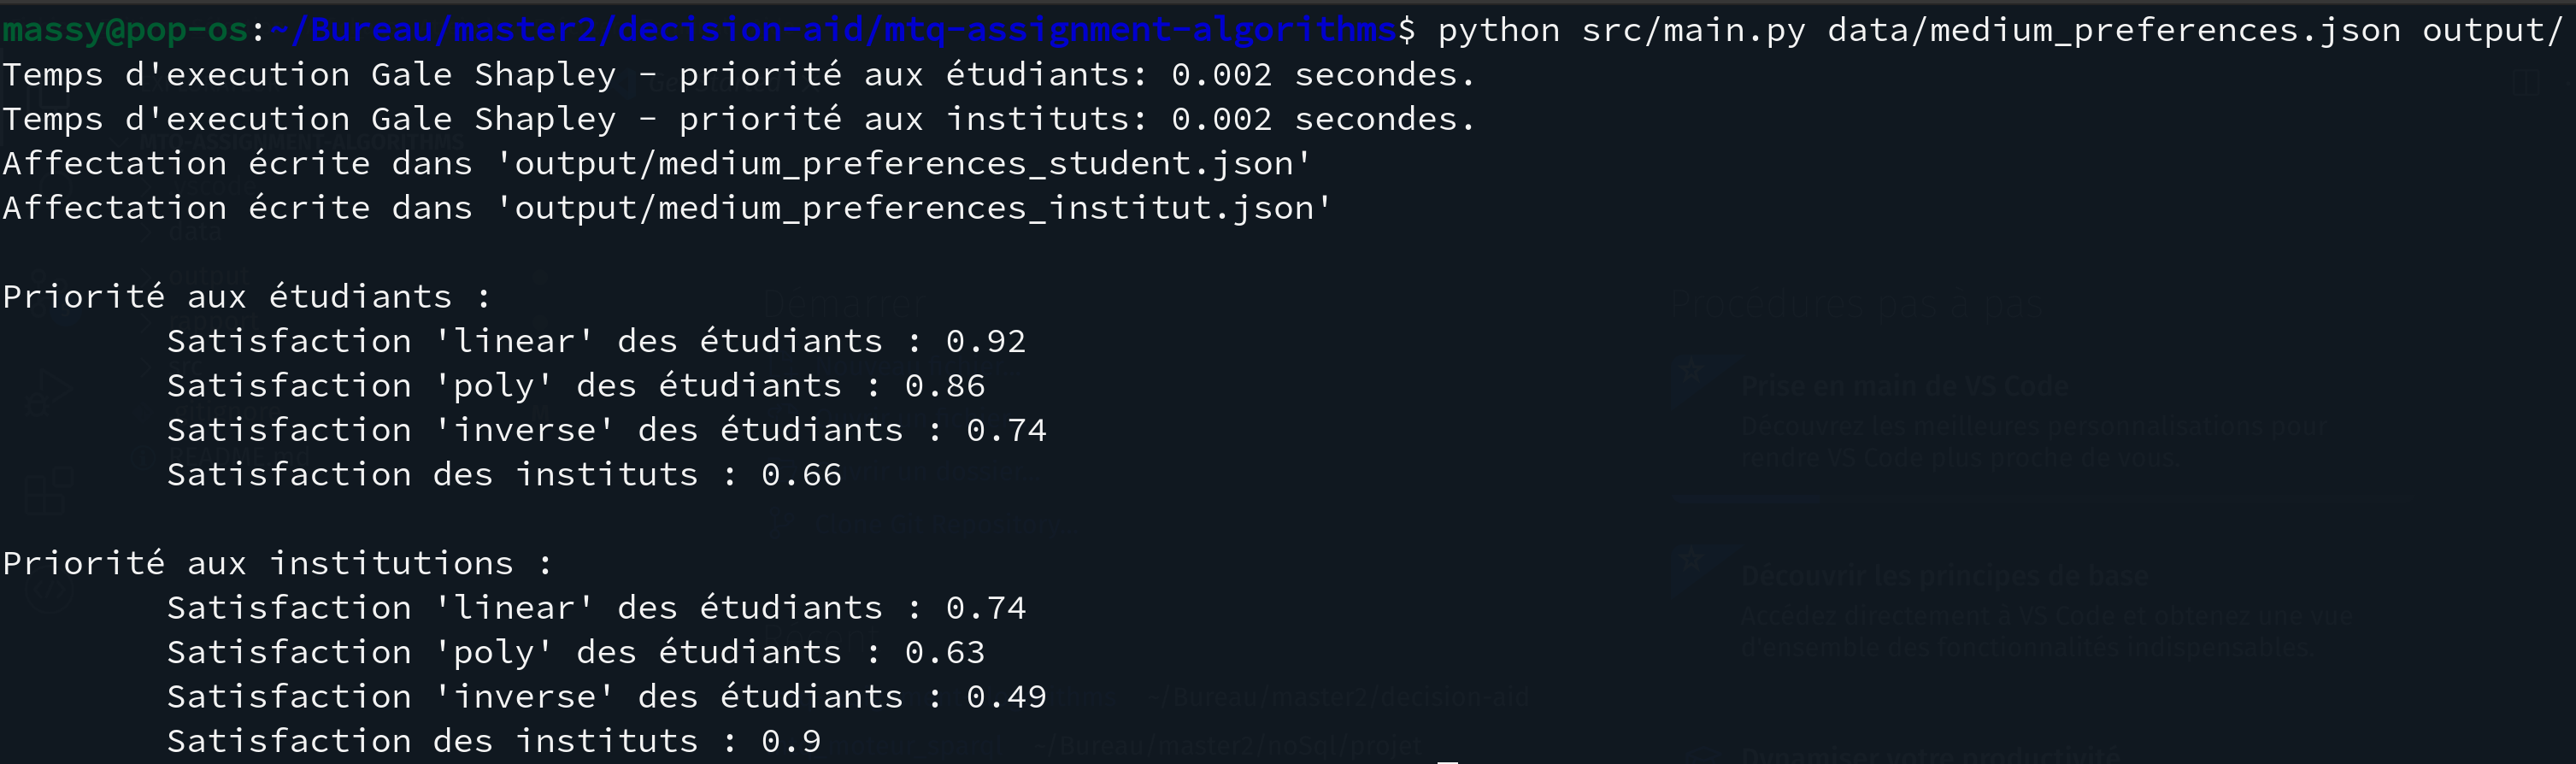
\includegraphics[width = 0.8\textwidth]{img/sortie_programme.png}
  \caption{Affichage produit par le programme principal}
  \label{fig:sortie}
\end{figure}

De plus, ce programme exporte dans deux fichiers sous le format \textit{JSON}\footnote{Le format \textit{CSV} est aussi possible mais pour la visualisation en graphe c'est le format \textit{JSON} qui est utilisé} les résultats des affectations (priorité aux étudiants et priorité aux institutions).

\begin{lstlisting}[language=json, caption="Fichier des affectations\, priorité au étudiants"]
  {
    "I1": ["E1", "E2", "E11"],
    "I2": ["E5", "E12", "E17", "E18", "E19"],
    "I3": ["E6", "E9", "E16", "E10"],
    "I4": ["E4", "E7", "E8", "E13", "E20"],
    "I5": ["E3", "E14", "E15"]
  }
\end{lstlisting}

\subsection{Interface de visualisation}

Pour pouvoir mieux visualiser les affectations des étudiants aux institution, on a pensé à une structure de graphes. Chaque institut et chaque étudiant sont représentés par un noeud étiqueté par leurs noms. Chaque affectation est représenté par une arête qui lie un étudiant à son institution.

\begin{figure}[!h]
  \centering
  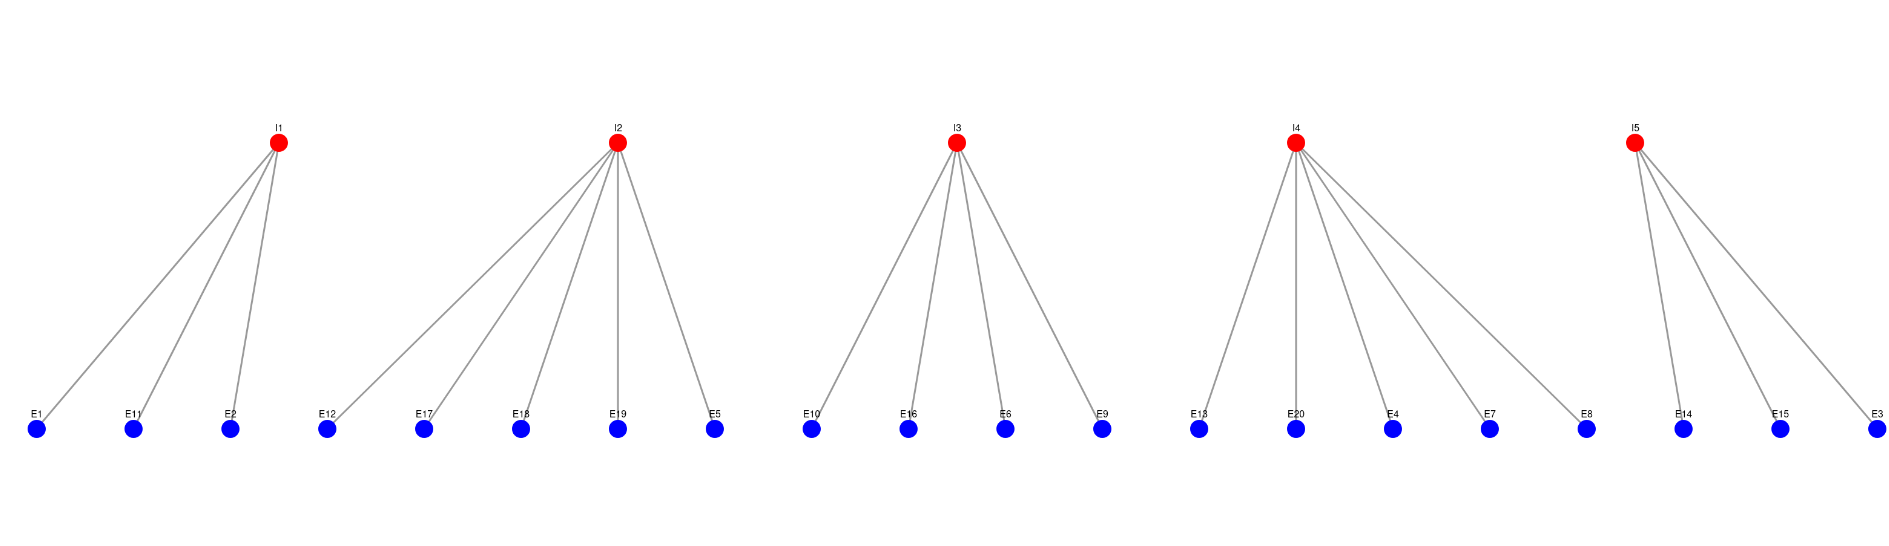
\includegraphics[width = 1.0\textwidth]{img/Screen_graph_dash.png}
  \caption{Visualisation en graphe}
\end{figure}

On obtient cette visualisation\footnote{Les points rouges représente les instituts et les points bleus représente les étudiants} en utilisant le programme \textit{graphviz.py} à qui en passe en argument un fichier \textit{JSON} produits precedement. Ce programme utilise la bibliothèque \textit{Dash}, qui permet de projeter des graphes interactifs via un petit serveur web en local.

\subsection{Méthodes de satisfaction}
La satisfaction de chaque côté est nécéssaire, pour évaluer nos algorithmes et les classés. Les problèmes de satisfaction apparaîssent toujours dans les systèmes d'aid à la décison ou plus précisement dans les systèmes d'affectations. Dans notre projet, on s'est concentré sur la satisfaction des étudiants, qui est un problème très fréquent dans la vie réelle. 
\subsubsection*{Satisfaction des étudiants}
Il existe plusieurs manières pour calculer la satisfaction des étudiants, on a choisi des méthodes qui sont significatives. Ces méthodes ont de même des points forts et des points faibles.
Toutes les méthodes sont faites, d'une façon à donner une note à chaque étudiant, selon son affectation par rapport à sa liste de préférences. Une moyenne de ces notes permet de mesurer la satisfaction globale de tout les étudiants. 
La note de chaque étudiant est comprise entre 0 et 1, c.à.d si un étudiant a eu son premier choix, il aura une note de 1 et s'il a eu son dernier choix, il aura une satisfaction égale à 0. Les notes des autres choix sont calculés avec des fonction mathématiques du genre $y = f(i)$, tel que, \textit{y} est la note de satisfaction et \textit{i} est la position de l'affectation de l'étudiant dans sa liste de préférences. 


\paragraph{Linéaire} En premier, une fonction linéaire, une façon très simple de calculer les satisfactions. Son principe est de donner une note à un choix \textit{i} d'un étudiant qui est infèrieure à la note du choix \textit{i-1}. Cette note diminue de 1 vers 0 d'une façon constante (comme le montre le graph ci-dessous) et cela selon le nombre de choix \textbf{k} des étudiants. Donc, par exemple si \textbf{k} = 10, on aura une liste de valeurs = (1, 0.9, 0.8 ,0.7, \dots, 0). 
Cette méthode de calculer est efficace pour un petit jeu de données, mais si on a un grand jeu de données, par exemple 100000 étudiant et 100 instituts, on a constaté que la satisfaction globale approche de 1, car les cinq premiers choix auront des notes élevées égales à (1, 0.99, 0.98, 0.97, 0.96), alors que dans un jeu de données pareil, 90\% des étudiants ont eu un de leurs trois premiers choix et que le pire étudiant a eu son 11ème choix avec une note de 0.9, tout cela affecte la moyenne globale des satisfactions et du fait quelle soit proche de 1. Aussi, vu que notre fonction diminue d'une façon linéaire, la différence entre la note du 1\textsuperscript{er} et du 2\textsuperscript{ème} choix est égale à la différence entre la note du 66\textsuperscript{ème} et du 67\textsuperscript{ème} choix. Ce qui nous a mener à penser à d'autres fonctions.

\begin{figure}[!h]
  \centering
  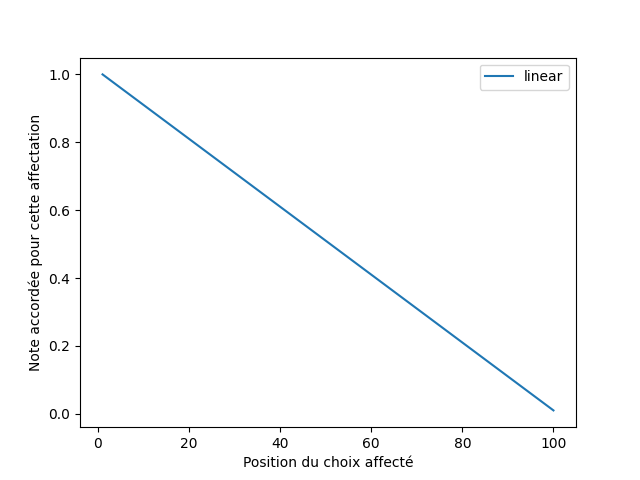
\includegraphics[width = 0.5\textwidth]{img/linear.png}
  \caption{Fonction linéaire}
\end{figure}

\paragraph{Polynomiale} Une fonction qui diminue d'une façon polynomiale, c.à.d, la différence entre  chaque deux choix décroît en allant du premier au dernier choix. ce qui limite le problème de la fonction linéaire. Par exemple, la différence entre la note du 1\textsuperscript{er} et du 2\textsuperscript{ème} choix est supèrieure à la différence entre la note du 66\textsuperscript{ème} et du 67\textsuperscript{ème} choix. Ce qui donne une forme d'importance aux premiers choix et une importance moindre aux derniers. Dans un cas pratique, un étudiant qui aura son 50\textsuperscript{ème} choix ou son 60\textsuperscript{ème} choix reste déçu dans les deux cas. Par contre, un étudiant qui aura son 1\textsuperscript{er} choix ou son 10\textsuperscript{ème}, voit sa satisfaction très affecter. Le graphe ci-dessous montre la décroissance non linéaire de la note d'une affectation. 

\begin{figure}[!h]
  \centering
  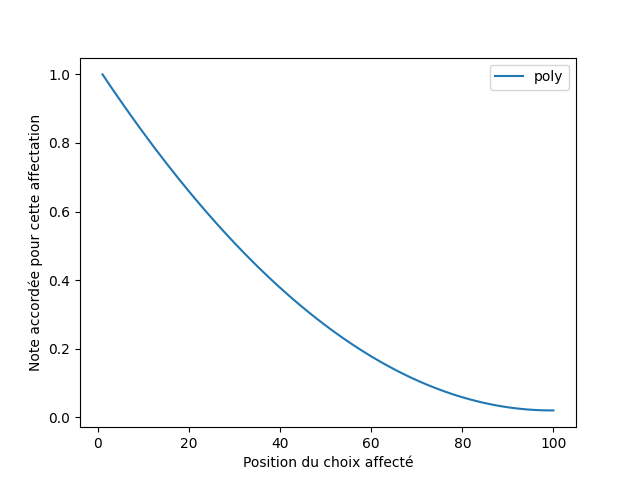
\includegraphics[width = 0.5\textwidth]{img/poly.png}
  \caption{Fonction polynomiale}
\end{figure}

\paragraph{Inverse} Une fonction inverse du genre $f(i) = \frac{1}{i}$. Cette fonction permet de donner une plus grande importance aux premiers choix, dans ce cas là le 2\textsuperscript{ème} choix aura une note de 0.5, qui est une différence énorme entre le 1\textsuperscript{er} et le 2\textsuperscript{ème} choix. on a pensé a cette fonction pour donner une satisfaction globale qui accorde plus d'importance au 1\textsuperscript{er} choix, Donc plus la moyenne est élevée, plus on saura qu'un grand nombre d'étudiants ont eu leurs 1\textsuperscript{er} choix. Le graphe ci-dessous montre la décroissance de la fonction inverse. 

\begin{figure}[!h]
  \centering
  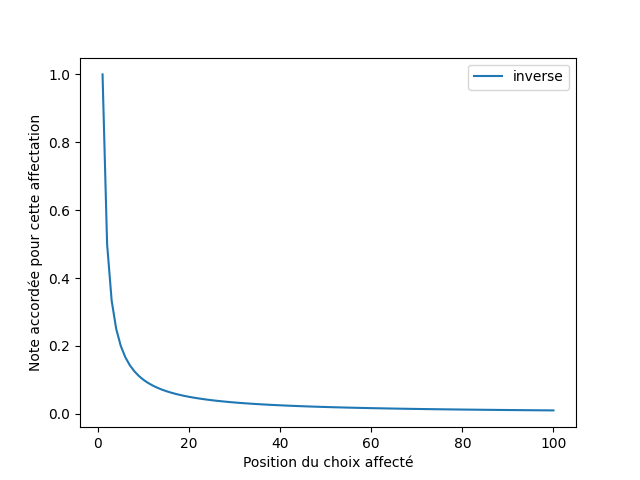
\includegraphics[width = 0.5\textwidth]{img/inverse.png}
  \caption{Fonction inverse}
\end{figure}

Nous pouvons remarquer, sur la figure ci-dessous, la différence entre ces différentes fonctions.

\begin{figure}[!h]
  \centering
  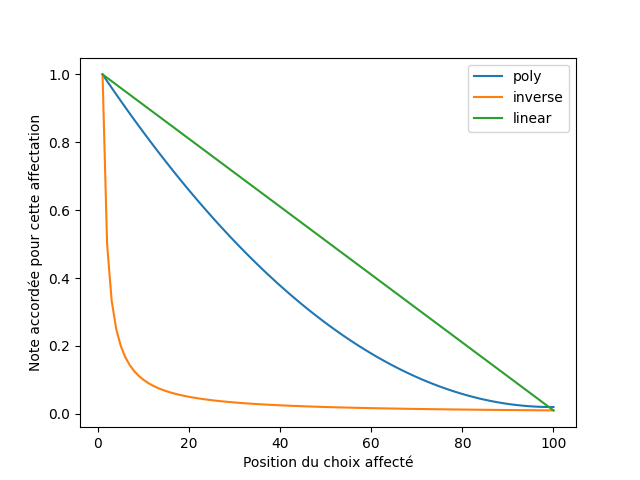
\includegraphics[width = 0.5\textwidth]{img/comparatif.png}
  \caption{Comparaison entre les fonctions}
\end{figure}

\subsubsection*{Satisfaction des instituts}
Contrairement à la satisfaction des étudiants, celle des institus doit réspecter une contrainte supplémentaire, qui est du au faite qu'on affecte à chaque institut plusieurs étudiants selon sa capacité $Q$. Pour palier à cette contrainte et avoir une valuer de satisfaction significative, Nous attribuons une note maximale de 1 pour un institut donné, si et seulement si les étudiants affectés à cet institut sont les $Q$ \textbf{premiers} choix de ce dernier. inversement, une note de 0 est attribué si et seulement si les étudiants affectés à cet institut sont les $Q$ \textbf{derniers} choix de ses préférences. Toutes les affectations qui sont au milieu suive une fonction qui diminue linéairement. Une moyenne est calculé pour avoir une satisfaction globale de tout les instituts.


\begin{figure}[!h]
  \centering
  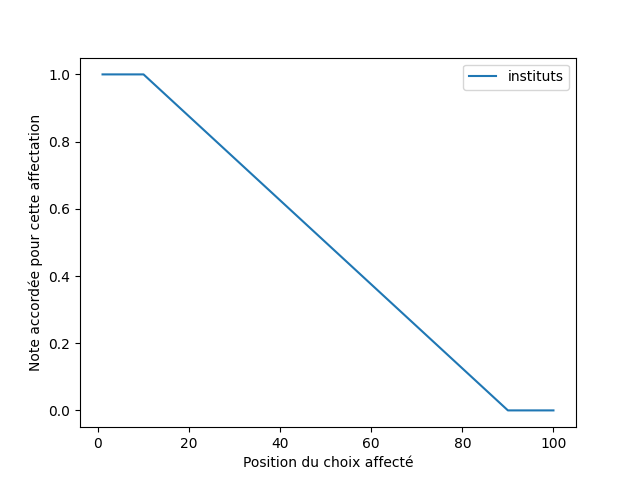
\includegraphics[width = 0.5\textwidth]{img/instituts.png}
  \caption{Fonction priorité aux instituts pour $Q = 10$}
\end{figure}

\begin{figure}
  
\end{figure}


\section{Extension du système}

\subsection{Random assignement}

\subsection{Li mkawda 3lihoum}

\section{Conclusion}

\subsection{Utilisation du programme}


\subsection{Perspectives}

\subsubsection{Pré-matching-Problem and Theroem de HALL}


\end{document}